\section{Inverse Kinematics}

\emph{Inverse Kinematics}, abbreviated as \emph{IK}, is a powerful method of control, with which the control problem of positioning the endpoint of a multiple DoF (Degree of Freedom) system can be solved. Here, the endpoint of the multiple DoF system is specified, and the control inputs for the system to achieve the endpoint are computed by the inverse kinematics algorithm.

This find wide application in systems like robotic arms, where the positioning of the arm endpoint can be specified, and joint angles can be computed for positioning the endpoint at the desired location. Similarly, it can be applied to the quadruped leg to compute the leg joint angles from a specified leg endpoint position.

In our quadruped robot, it is used to solve for the three joint angles in each of the four legs, making up a 12 DoF system. Here, we use a [\emph{Hip, Shoulder, Elbow}] nomenclature, which, we admit, is not anatomically accurate. For us, however, it seemed intuitive to think of it in such a way, and thus will continue to use it through the derivation below. The angles are, namely:

\begin{center}
    \(\theta_0 : \) hip joint angle\\
    \(\theta_1 : \) shoulder joint angle\\
    \(\theta_2 : \) elbow joint angle\\
\end{center}

% Insert leg diagrams/figures here
\begin{figure}
    \begin{multicols}{2}
        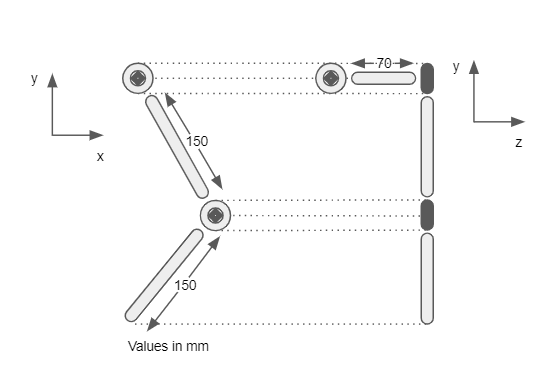
\includegraphics[width=0.5\textwidth]{legFrontSideViewIK}
        \caption{\small Leg views from front, side}
        \label{fig:legViewsIK}
        
        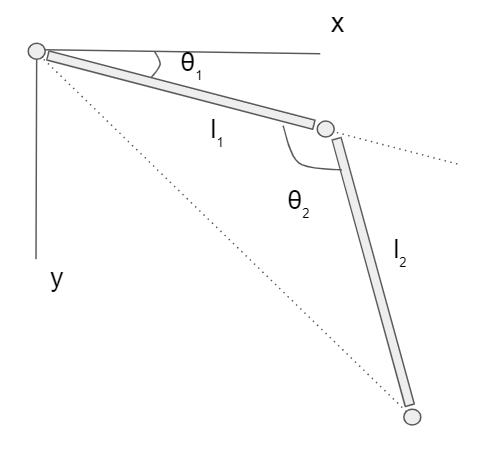
\includegraphics[width=0.3685\textwidth]{legSideViewAnglesIK}
        \caption{\small Annotated side view}
        \label{fig:sideViewAnnIK}
    \end{multicols}     
\end{figure}

Here, we derived our own inverse kinematics algorithm using trigonometric principles, a summary of which is given below.

The notations used in the figures are given below:

\begin{flushleft}
\(x = \) position of the leg endpoint along the x axis\\
\(y = \) position of the leg endpoint along the y axis\\
\(z = \) position of the leg endpoint along the z axis\\
\(l_0 = \) length of leg segment from hip to shoulder\\
\(l_1 = \) length of leg segment from shoulder to elbow\\
\(l_2 = \) length of leg segment from elbow to foot\\
\(l_3 = \) length of front projection from hip to foot\\
\(l_4 = \) length of front projection from shoulder to foot\\
\(r = \) projected leg length from shoulder to foot\\
\(\theta_0 = \) hip joint angle\\
\(\theta_1 = \) shoulder joint angle\\
\(\theta_2 = \) elbow joint angle\\

\end{flushleft}

For the purpose of deriving the relationships of these parameters to the joint angles \(\theta_0\), \(\theta_1\), and \(\theta_2\), we define

\begin{flushleft}
\(\theta_{1 \ effective} = \) effective angle between \(l_3\) and the x axis
\end{flushleft}

% Add annotated front view figure
From Figure \ref{fig:sideViewAnnIK} and Figure, we get \(l_3\) and \(l_4\) as
\[l_3 = \sqrt{y^2 + z^2}\]
\[l_4 = \sqrt{l_3^2 + l_0^2}\]

Now, \(r\) can be found to be
\[r = \sqrt{x^2 + l_4^2}\]

Then, we can compute the hip angle \(\theta_0\) as
\[\theta_0 = \arccos{\left( \frac{z l_0 + y l_4}{l_3^2} \right)}\]

Solving for the knee angle, \(\theta_2\)
\[\cos{\theta_2} = \frac{l_1^2 + l_2^2 - r^2}{2 l_1 l_2}\]

Thus, the knee angle, \(\theta_2\) is given by
\[\theta_2 = \arccos{\left( \frac{l_1^2 + l_2^2 - r^2}{2 l_1 l_2} \right)}\]

Now, we need to solve for the shoulder angle \(\theta_1\). For this,
\[\theta_{1 \ effective} = \arctan{\left( \frac{l_4^2}{x^2} \right)}\]


